\section{Results} \label{chap:results}

This evaluation is computed using recordings never available as training data.
The training pipeline is deterministic, meaning that all randomly generated
numbers follow the same seed unless otherwise specified. Nevertheless, when the
frame duration or the segment length is changed, the produced datasets have a
different number of samples. Comparing the performance of models trained using
datasets with different sizes can lead to wrong conclusions.


\subsection{Metrics} \label{sec:metrics} This work measures the performance of
the trained models using commonly used odometry and simultaneous localization
and mapping metrics: \cite{Measuring2019}.

\subsection{Selected model} \label{sec:selected-model}

After the experiments listed in \cref{sec:results-experiments} this work
selects a model trained on a dataset of segments of 50 frames, each of them
spans over 15 ms and has 64 features from a single
\nameref{para:gammatone-filterbank} extractor. The extractor is applied on
the average of the audio signal channels with a frequency range of [50, 80000]
Hz and features on te Bel scale. Training data from all available recordings is
selected using the \texttt{with-laptop} strategy split described in
\cref{table:training-data-split}, a \nameref{para:model-task-ord-class} task
with 28 different linearly distributed longitudinal velocity ranges and a
\nameref{para:model-arch-norm-cnn} architecture with a small size described as
\texttt{S} in \cref{table:model-arch-sizes}. 

\Cref{table:results-selected-model} shows the average performance of the
selected model across all seven evaluation recordings and devices.
\Cref{fig:high-slip} shows the its results on an evaluation recording
characterized by high slippage driving conditions using two different devices.

\begin{table}
    \centering
    \begin{tabular}{|c|c|c|}
        \hline
                          & Mean ATE [m] & Mean RPE [m/s] \\ \hline
        Acoustic Odometry & $1.02e-03$   & $5.10e-03$     \\
        \hline
    \end{tabular}
    \caption[Selected model average performance across evaluation recordings
        and devices]{Selected model average performance across all evaluation
        recordings and all devices. \nameref{para:ATE} is computed between
        frames with a duration of 15 ms and \nameref{para:RPE} is computed
        using time windows 1s long.}
    \label{table:results-selected-model}
\end{table}


\begin{figure}
    \centering
    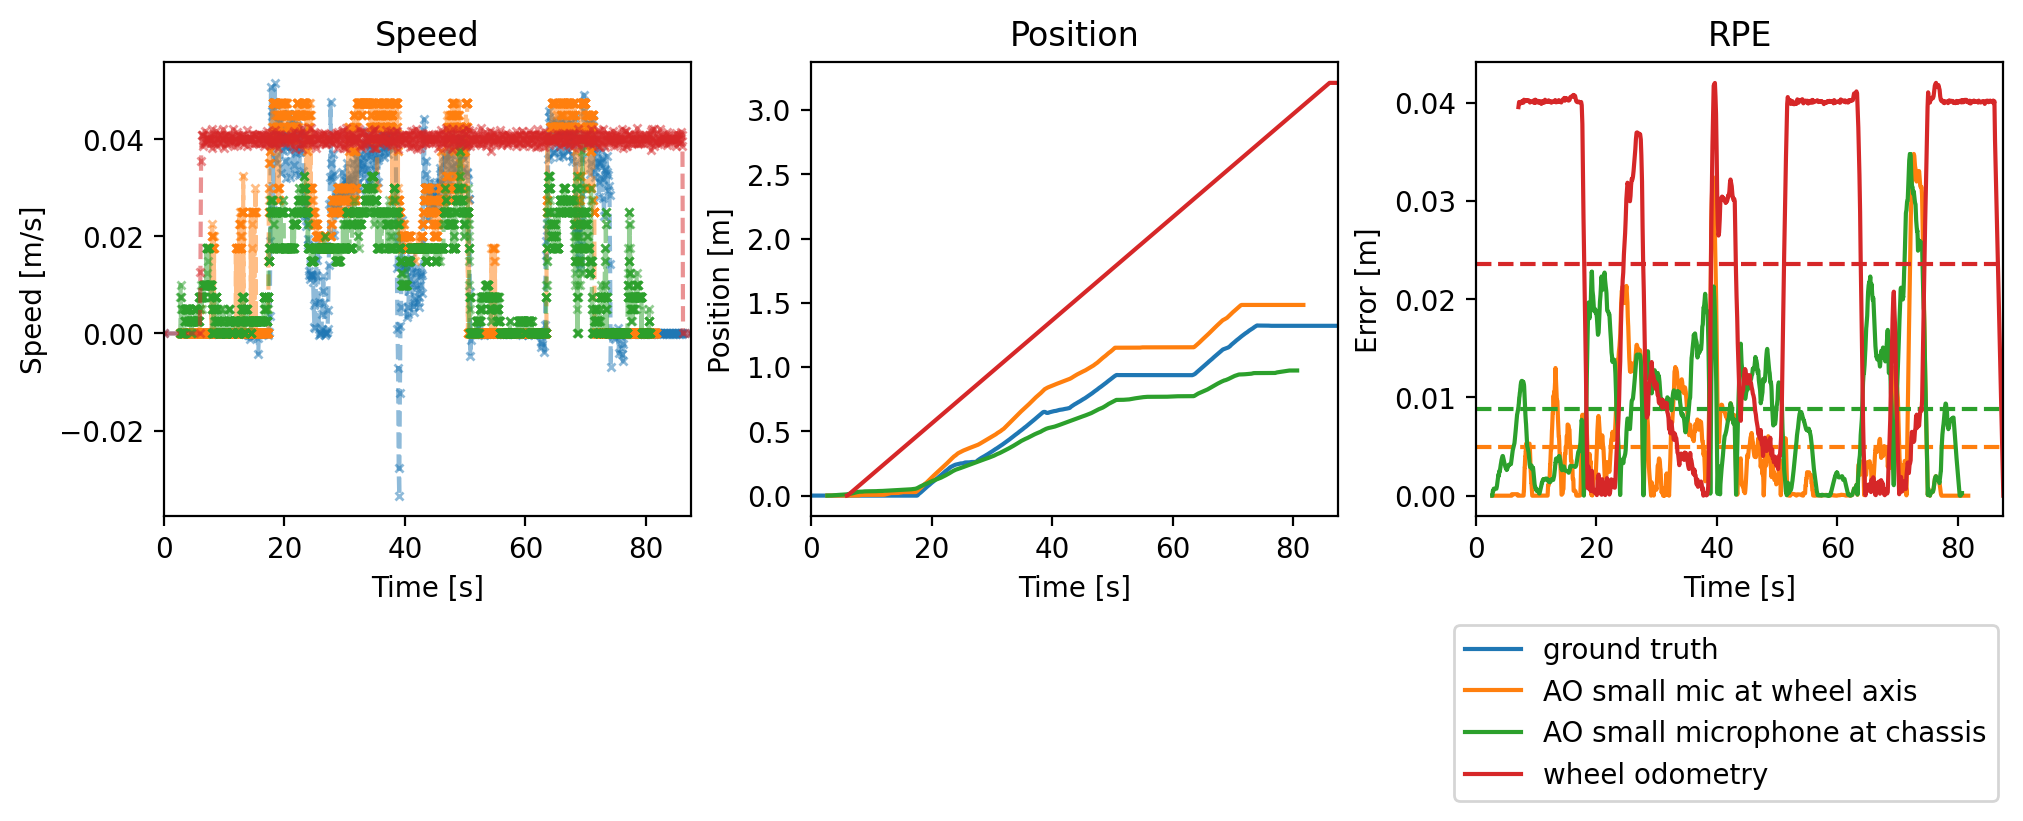
\includegraphics[width=0.95\textwidth]{\subdir/high-slip.png}
    \caption[Selected model on high slippage conditions]{Selected model
        evaluated on a recording characterized by high slippage conditions
        using two different devices.}
    \label{fig:high-slip}
\end{figure}

\paragraph{Noise} One can see in \cref{fig:noise-effect} the behavior of the
selected model against white noise. Generally, white noise increases the value
of the estimated motion. Very small values of signal-to-noise ratio (-20 dB,
which is a noise power 100 times higher than the signal) impede the model to
recognize situations where the wheel is not moving.

\begin{figure}
    \centering
    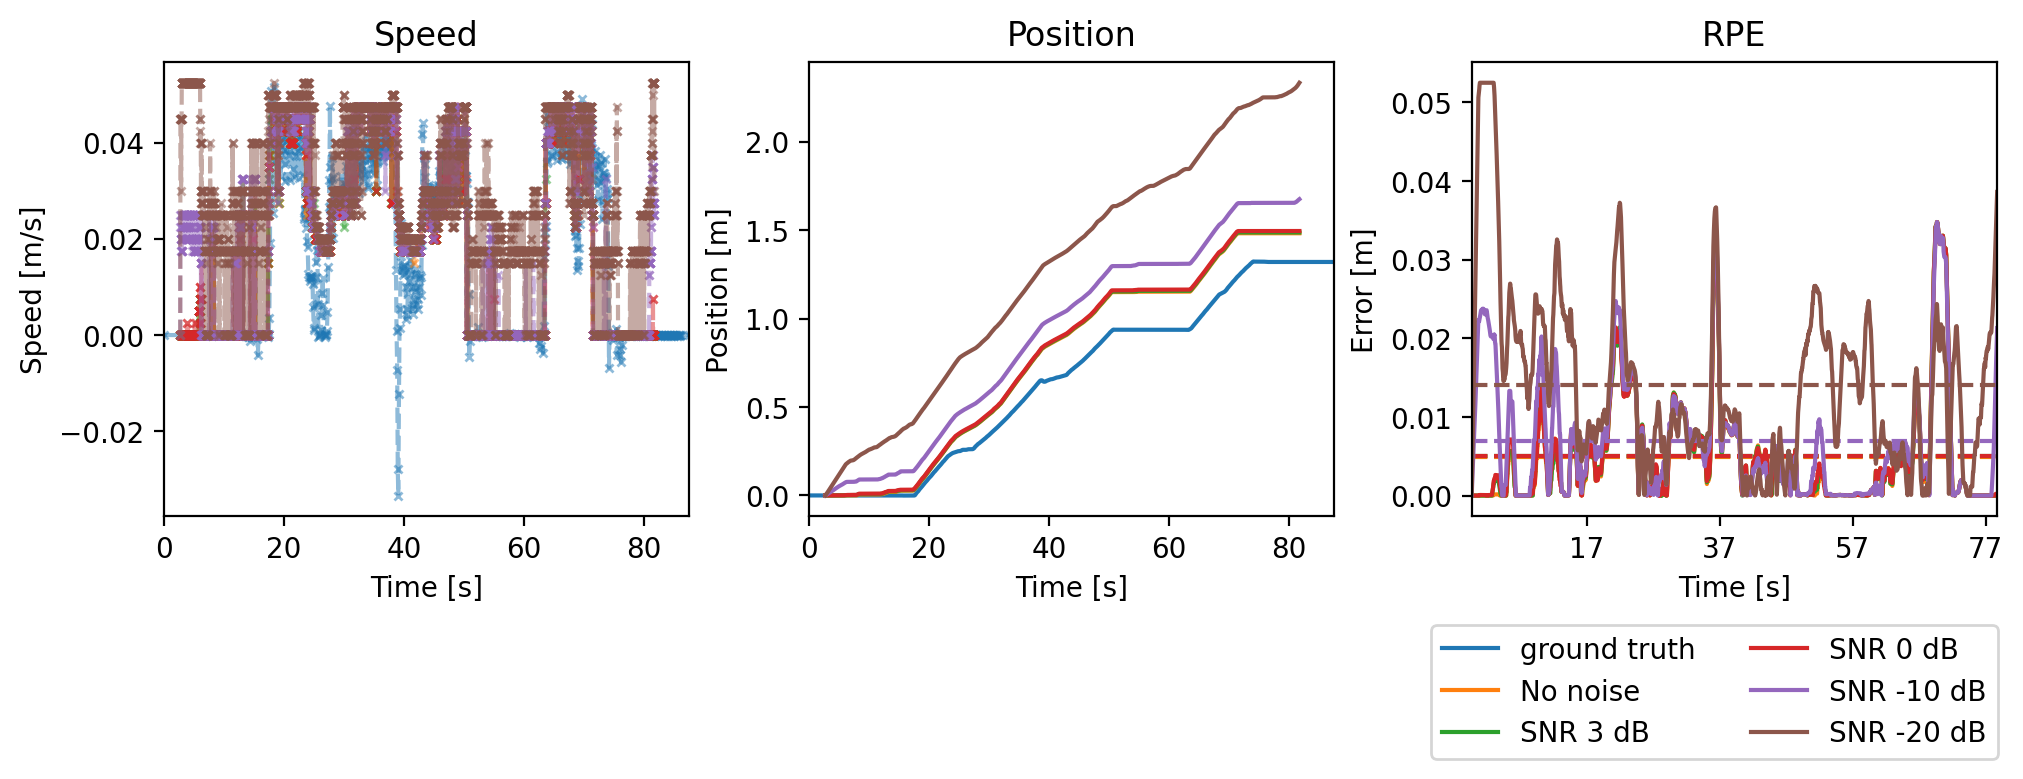
\includegraphics[width=\linewidth]{\subdir/noise-effect.png}
    \caption[Selected model with white noise]{Selected model evaluated on a
        recording with added white noise with varying signal-to-noise Ratio
        values.}
    \label{fig:noise-effect}
\end{figure}

\paragraph{Computational cost} Tests with the selected model on a CPU show that
the time to compute the feature extraction is a 40\% of the total time to
process a new frame, which is 2.03 ms on an Intel\textregistered{}
Core\texttrademark{} i7-9750H CPU at 2.60GHz. The prediction time takes up a
55\% of the total time while the remaining 5\% corresponds to loading the new
frame into memory The system is able to run 7.5 times faster than real time on
this particular hardware. Using hardware acceleration with CUDA the total time
to process a new frame is slightly lower: 1.93 ms on a NVIDIA GeForce RTX
2060 GPU.

\paragraph{Compared with other models} The selected model is evaluated against
two other odometry methods: Wheel odometry computed from the ground truth wheel
angular speed; Visual SLAM using Intel\textregistered{}
RealSense\texttrademark{} Tracking Camera T265, which is based on visual
odometry. \Cref{fig:other-methods} is the evaluation in an undisturbed scenario
for all methods, no acoustic noise and no lightning changes or dynamic objects.
It shows that the selected model can perform with an accuracy comparable to
state-of-the-art commercial visual-based methods in this simplified scenario.
\Cref{fig:VO-challenge} instead corresponds to a scenario that is challenging
for visual odometry. Dynamic objects are moved in the camera field of view and
lightning conditions are changed during the recording. One can see in this
evaluation that the vulnerabilities of audio-based odometry and visual-based
odometry do not overlap. Which makes Acoustic Odometry more accurate in certain
scenarios where the visual odometry vulnerabilities are exploited.

\begin{figure}
    \centering
    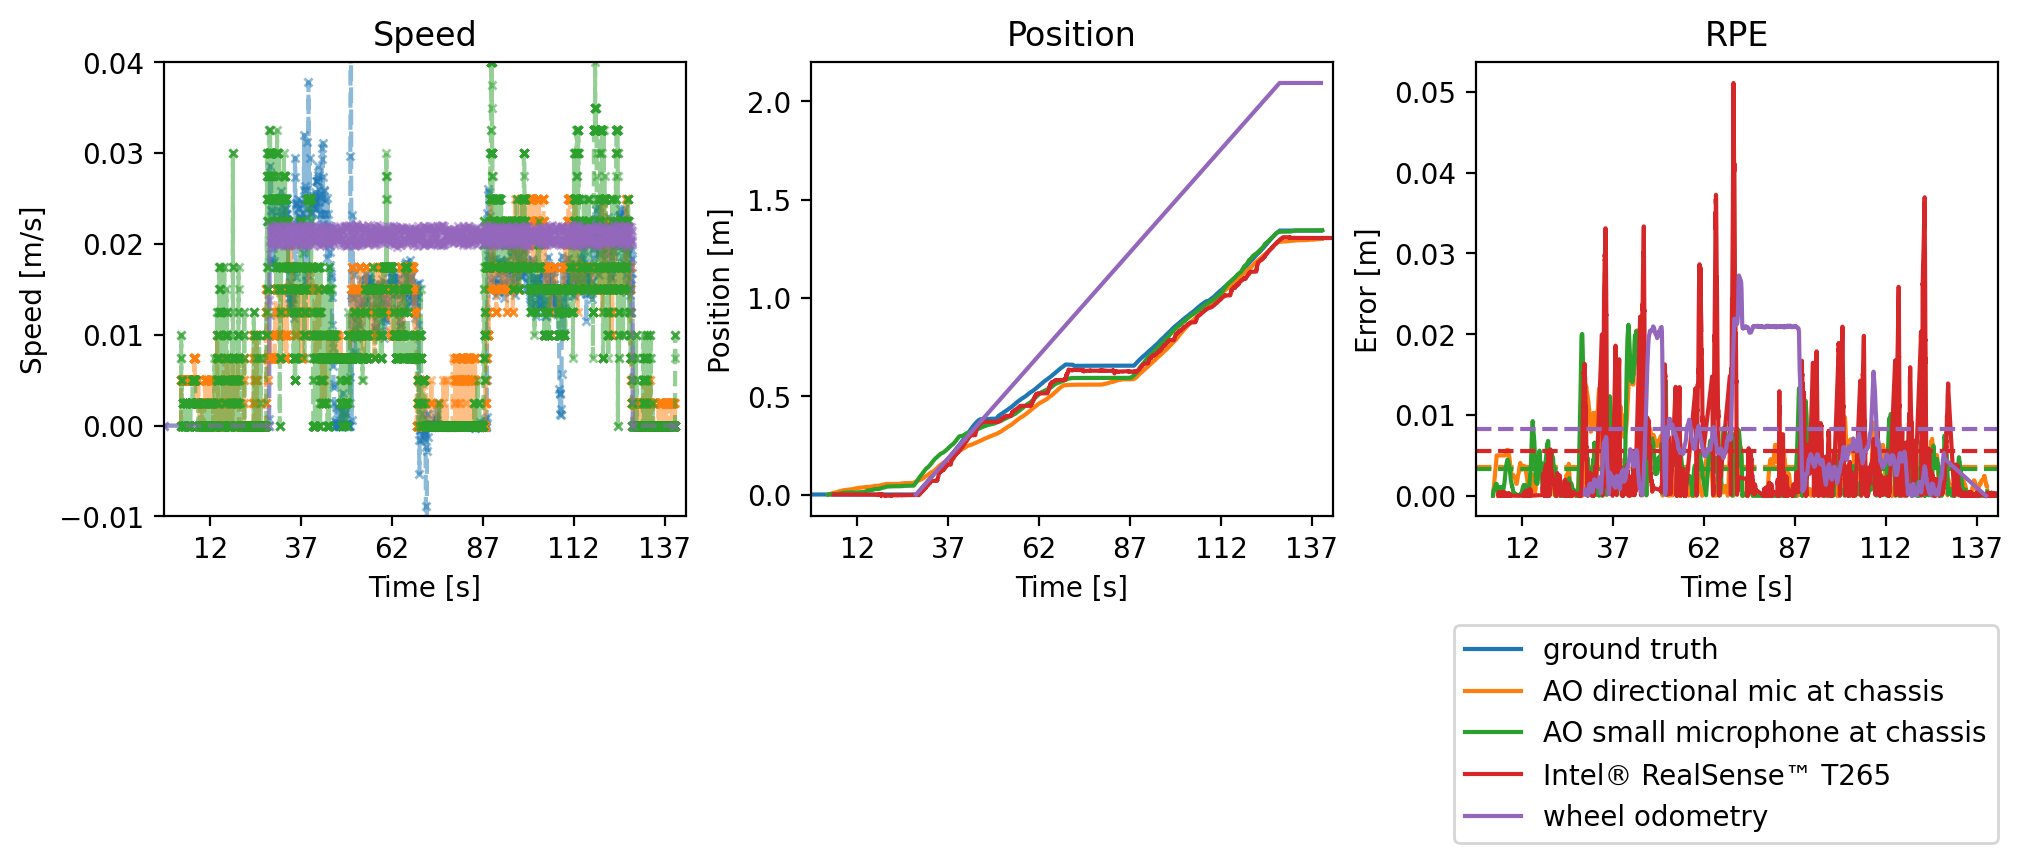
\includegraphics[width=\linewidth]{\subdir/other-methods.png}
    \caption[Selected model compared to other methods]{Selected model evaluated
        evaluated against Visual SLAM (based on visual odometry) and wheel
        odometry.}
    \label{fig:other-methods}
\end{figure}

\begin{figure}
    \centering
    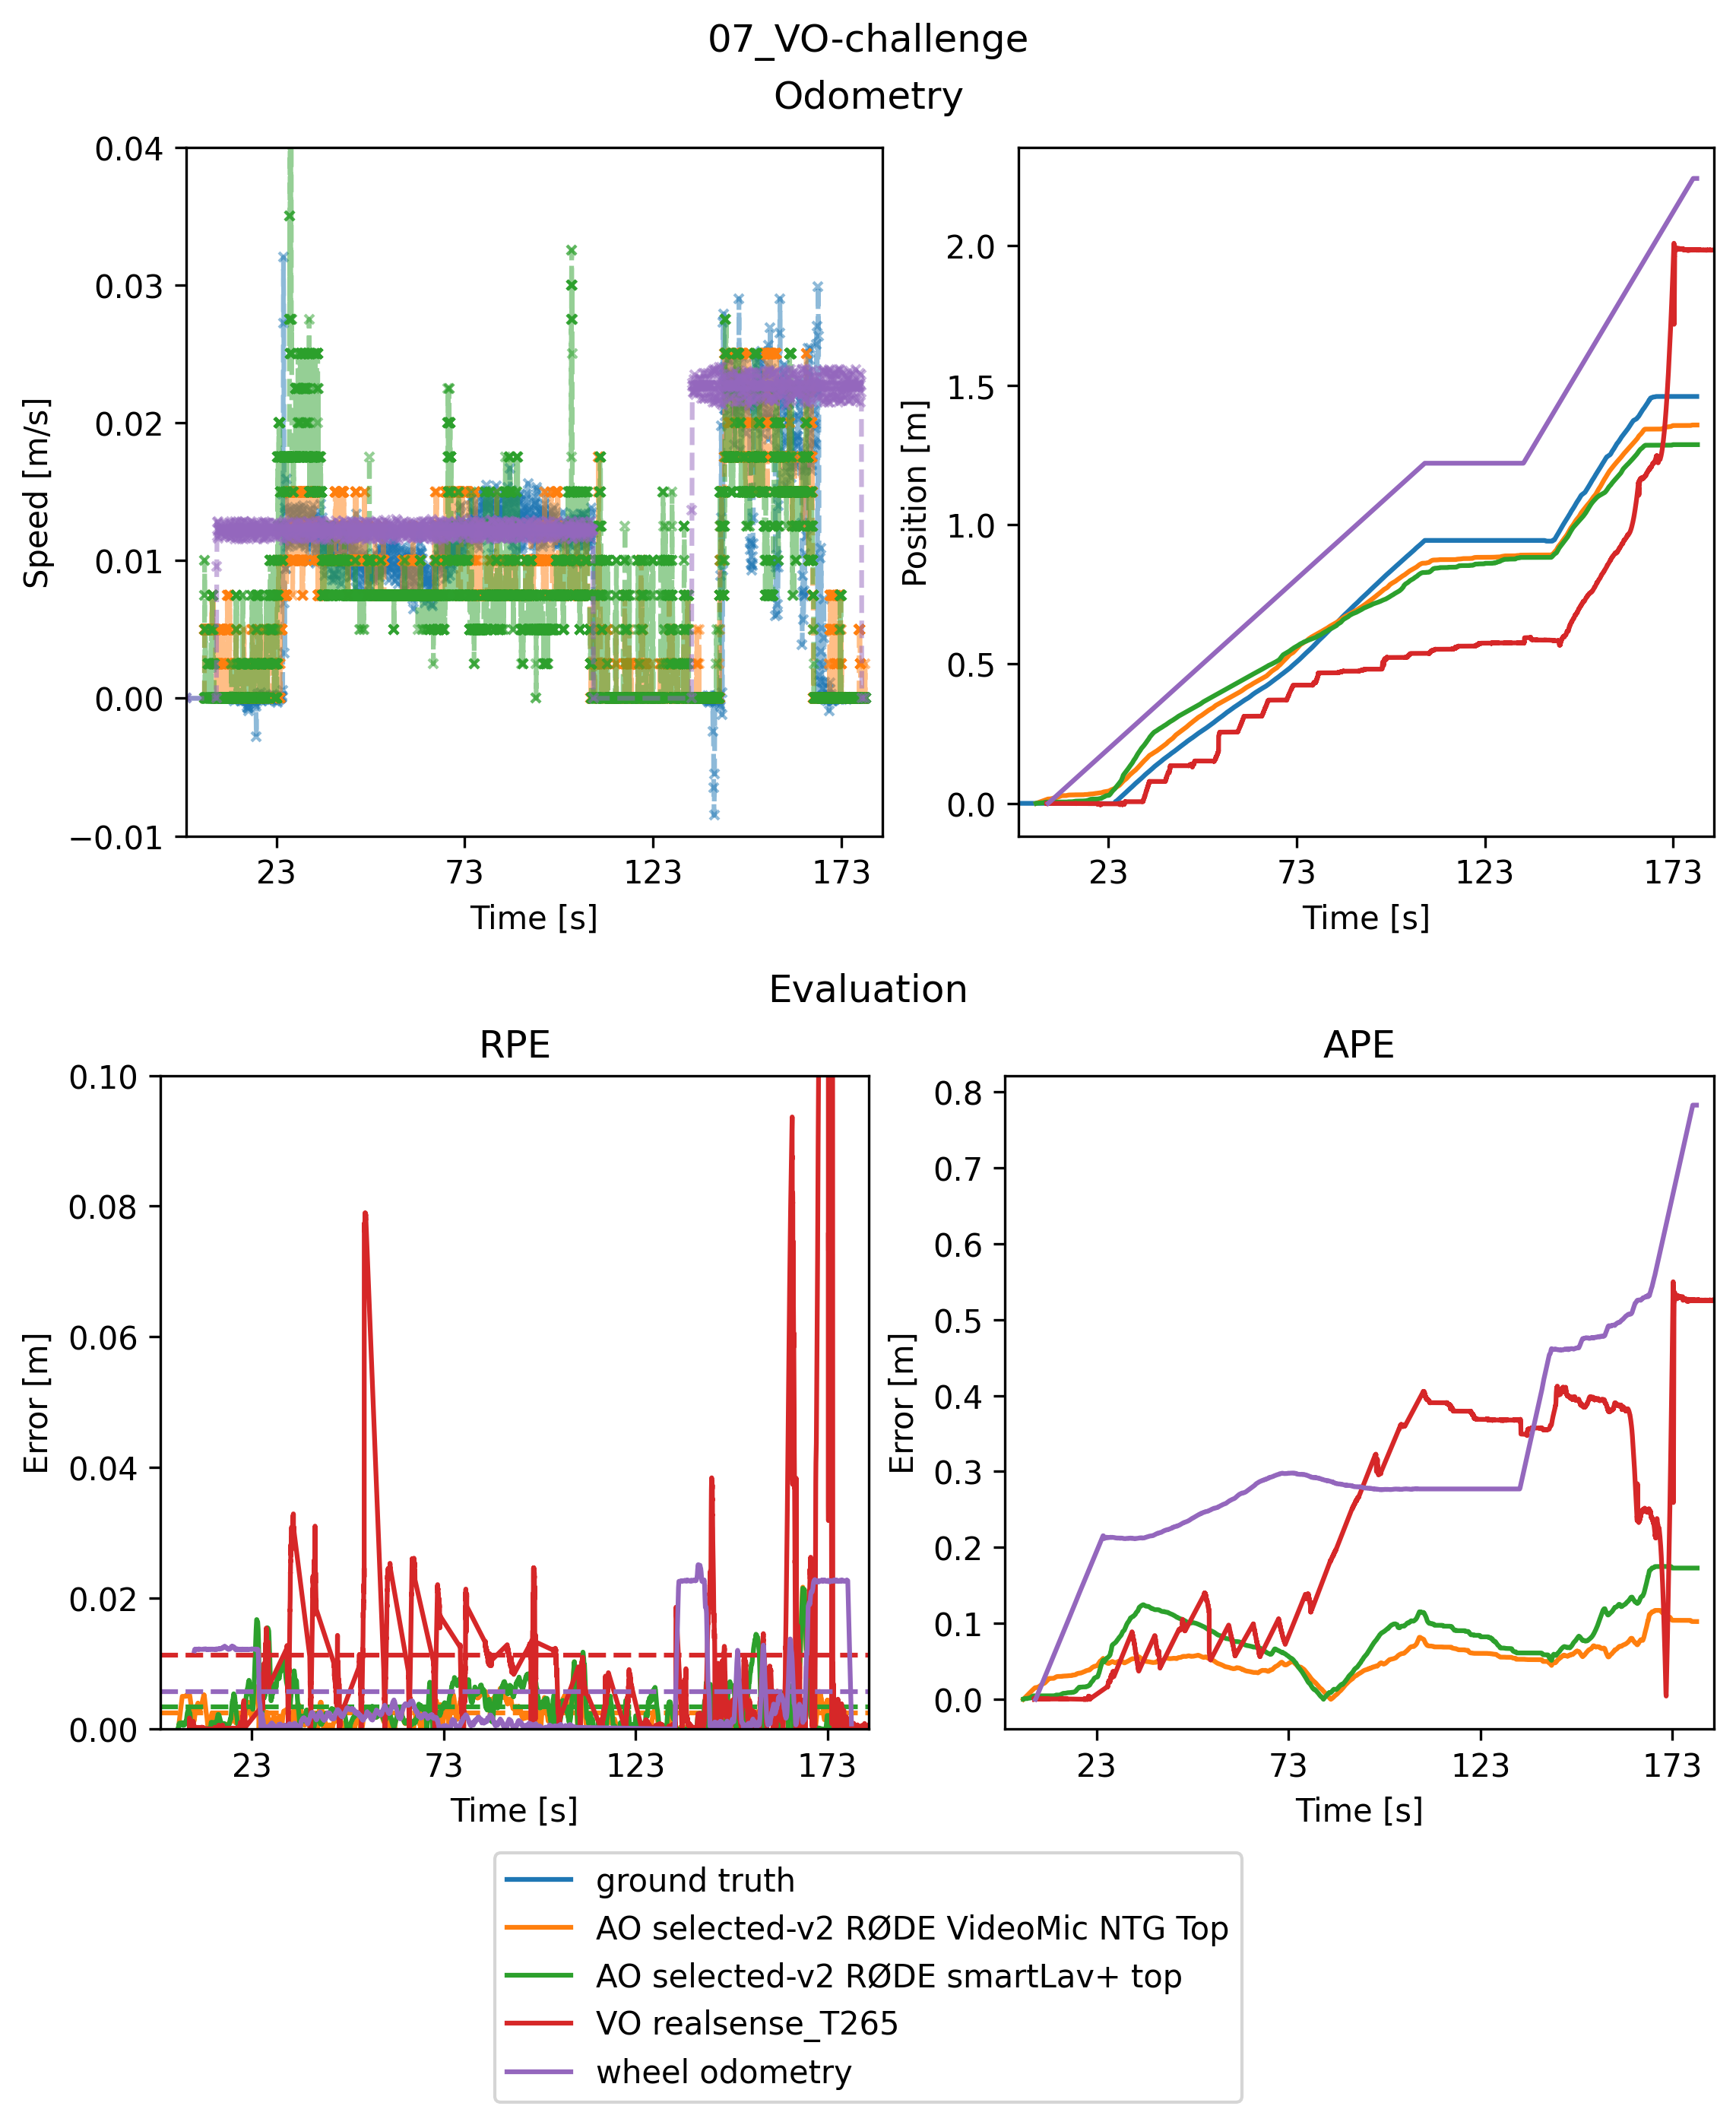
\includegraphics[width=\linewidth]{\subdir/VO-challenge.png}
    \caption[Selected model on a challenging scenario for Visual Odometry]{
        Selected model evaluated against Visual SLAM (based on visual odometry)
        in a scenario where visual odometry vulnerabilities are exploited:
        Dynamic objects are moved in the camera field of view and lightning
        conditions are changed during the recording.}
    \label{fig:VO-challenge}
\end{figure}

\include*{\subdir/discussion}